\section{Gearbox Design}
\subsection{Choosing reduction ratio}
The step angle of the stepper motor is equal to $1.8\,\degree$ (see \cref{tab:stepper_motor_params}). 
An angle of $0.1\,\degree$ was selected as the base output step angle of the platform, since it lets all angles featured in \cref{tab:best_combinations} be represented as integer multiples of this value, meaning a bigger step will be artificially achieved by stepping a couple of times with a smaller step.
That means that a reduction ratio 18:1 has to be achieved. 
DRV8825 stepper motor driver\footnote{\url{https://www.ti.com/lit/ds/symlink/drv8825.pdf}} which is used in this project allows for a reduction ratio up to 32:1 to be achieved via microstepping. A reduction ratio of 2:1 was chosen here, since higher microstepping ratios come with a reduced accuracy of the output \cite[sec.~Texas Instruments DRV8825]{by_HowAccurateMicrostepping_2016}.
That leaves 9:1 reduction ratio to be obtained using a gearbox.
\subsection{Gearbox Design Selection}
\subsubsection{Belt Drive}
A belt drive is a mechanical transmission system in which rotational motion is transferred between pulleys using a flexible belt. The ratio of pulley diameters determines the reduction ratio. In case of toothed belts, gears could be used instead of pulleys to minimise slipping. An example of a 3D-printed belt drive mechanism can be found in \cite[sec.~Belt Drive]{dejan_WhatBEST3D_2025}
\begin{figure}[H]
    \centering
    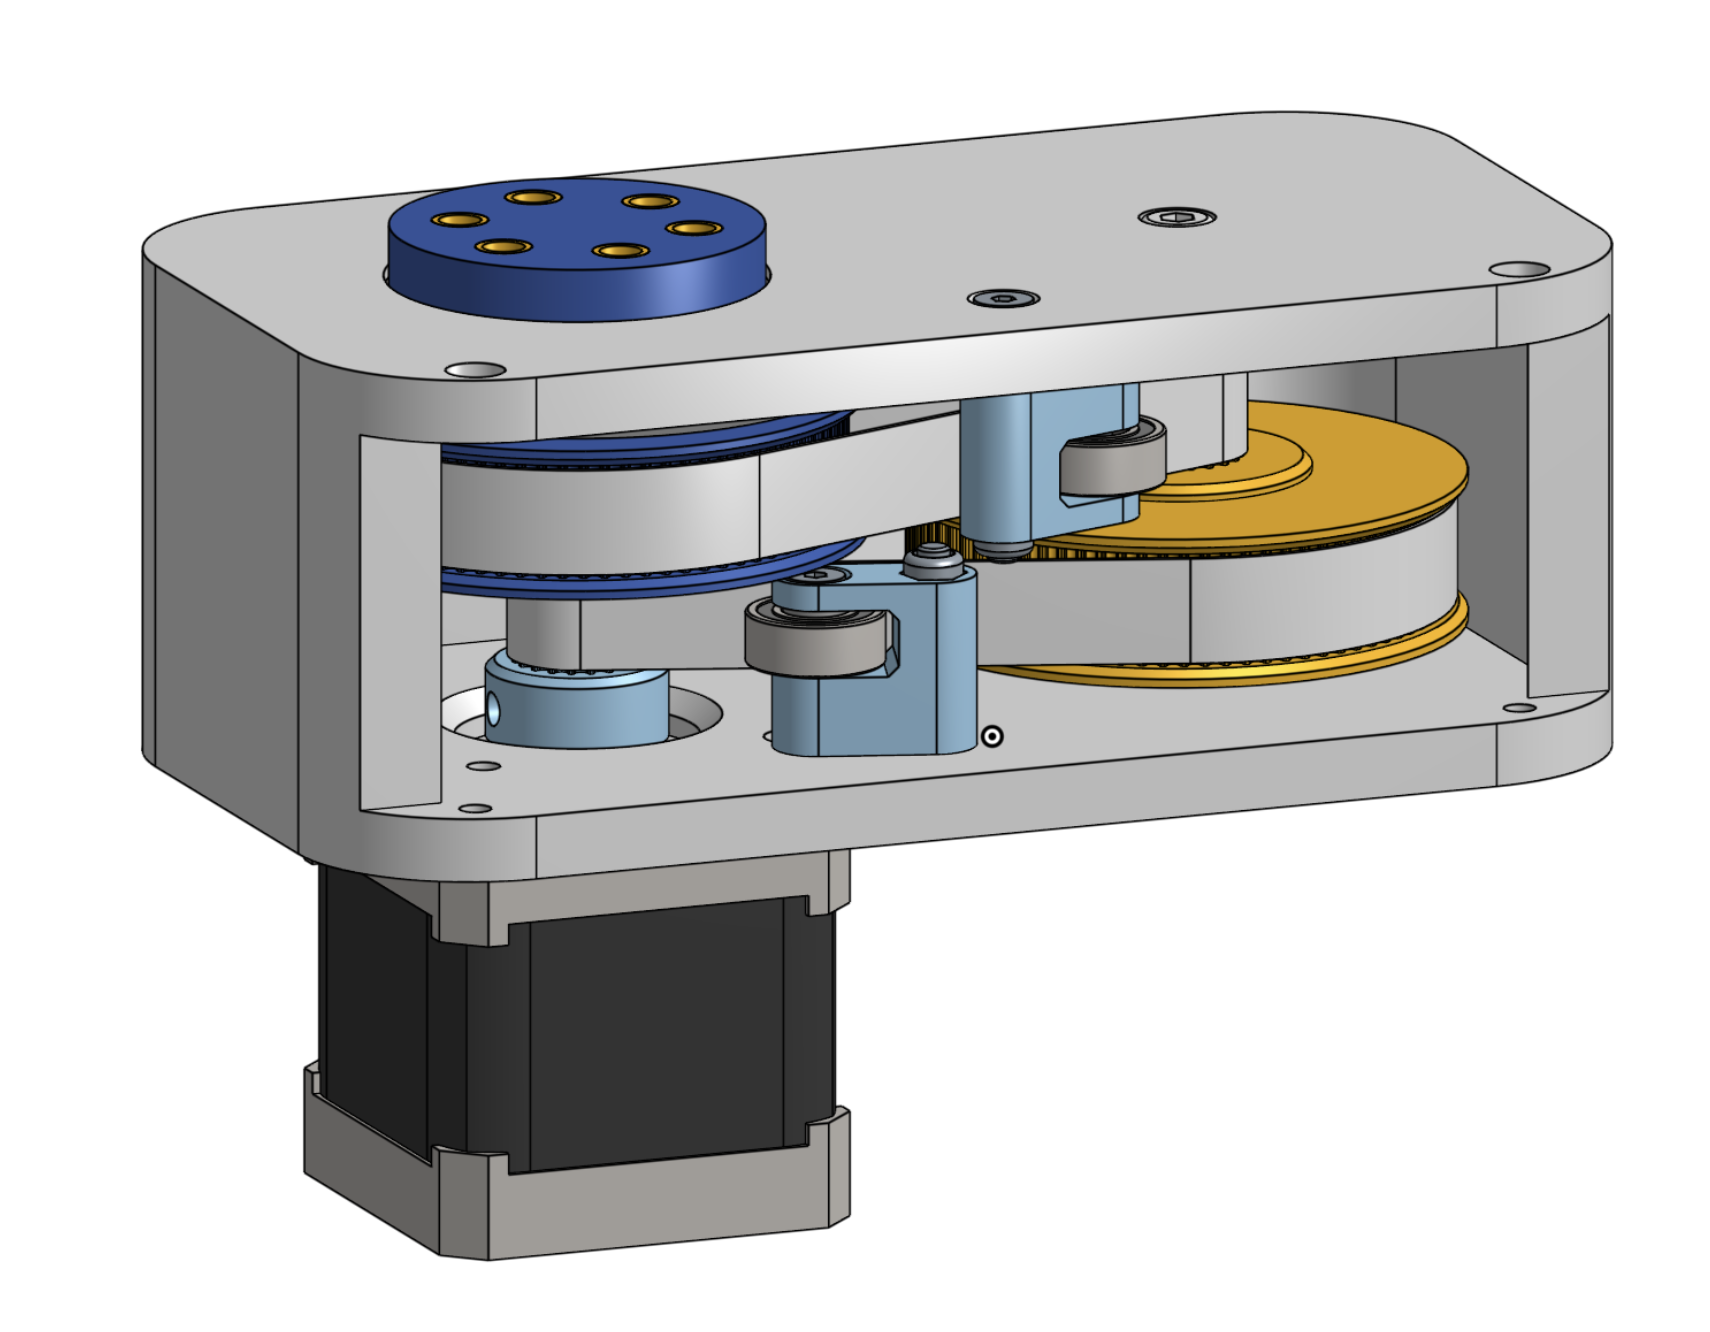
\includegraphics[width=0.6\textwidth]{design/gearbox_design/belt_drive.png}
    \caption{Belt drive featured in \cite{dejan_WhatBEST3D_2025}}
    \label{ph:belt_drive}
\end{figure}
\begin{tabular}{p{0.5\linewidth} p{0.45\linewidth}}
    \textbf{Pros} & \textbf{Cons} \\
    \begin{itemize}[label=\textcolor{green!60!black}{\textbf{+}}]
        \item Using belt ensures smooth and quiet operation that is hard to achieve with direct teeth-to-teeth contact in interlocking gears
    \end{itemize}
    &
    \begin{itemize}[label=\textcolor{red!70!black}{\textbf{--}}]
        \item The asymmetric mechanical arrangement, although compact overall, could obstruct the field of view of the \gls{lidar} sensor unless the scanning platform positions it excessively high above the drive mechanism. The symmetric designs presented next do not require such an elevated platform.
    \end{itemize}
\end{tabular}

\subsubsection{Cycloidal Gearbox}
A cycloidal gearbox is widely used in robotics and machining due to its low backlash\footnote{(dict.)Backlash -- the play between adjacent movable parts (as in a series of gears)} and its ability to provide exceptionally high reduction ratios and torque in a compact form factor \cite{qi_DesignPrincipleNumerical_2024}. A 3D-printed implementation and further discussion of its properties can be found in \cite{dejan_WhatCycloidalDriver_2021}.
\begin{figure}[H]
    \centering
    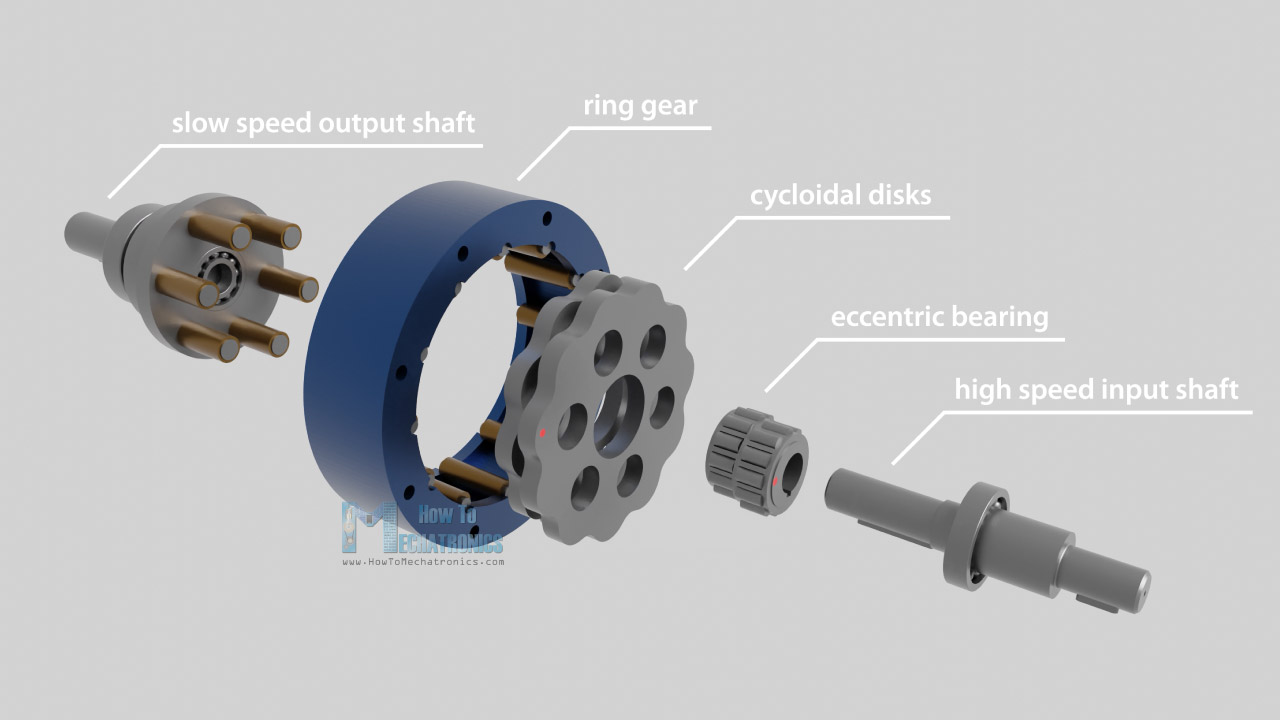
\includegraphics[width=\textwidth]{design/gearbox_design/cycloidal_drive.jpg}
    \caption{Photo of the components of cycloidal gearbox. Illustration taken from \cite{dejan_WhatCycloidalDriver_2021}}
    \label{ph:cycloidal_drive}
\end{figure}
\begin{tabular}{p{0.45\linewidth} p{0.45\linewidth}}
    \textbf{Pros} & \textbf{Cons} \\
    \begin{itemize}[label=\textcolor{green!60!black}{\textbf{+}}]
        \item Symmetric design (a requirement for our project)
        \item High reduction ratio in a compact space
    \end{itemize}
    &
    \begin{itemize}[label=\textcolor{red!70!black}{\textbf{--}}]
        \item Correct design of this system requires working with complex parametric equations inside CAD software to correctly design the movement of disks in a cycloidal manner (hence the name). Although CAD tutorials and design tools exist \cite{younis_BuildingCycloidalDrive_}, the design process remains cumbersome.
        \item High component count due to the large number of rollers required for high reduction ratios. In our case, a cycloidal gearbox with a 9:1 reduction ratio would require 10 ball bearings for each of the two cycloidal disks, making the design unnecessarily complex for an amateur project.
    \end{itemize}
\end{tabular}

\subsubsection{Planetary gearbox}
\label{subsubsec:planetary_gearbox}
A planetary gearbox is a compact symmetric transmission system consisting of a sun gear, planet gears, and an outer ring gear. They are widely used in automotive transmissions because multiple gear ratios can be achieved within a compact arrangement by selectively locking or driving different transmission components \cite[p. 158-159]{naunheimer_AutomotiveTransmissionsFundamentals_2011}. 3D-printed implementation can be seen in \cite{dejan_HowPlanetaryGears_2023}.
\begin{figure}[H]
    \centering
    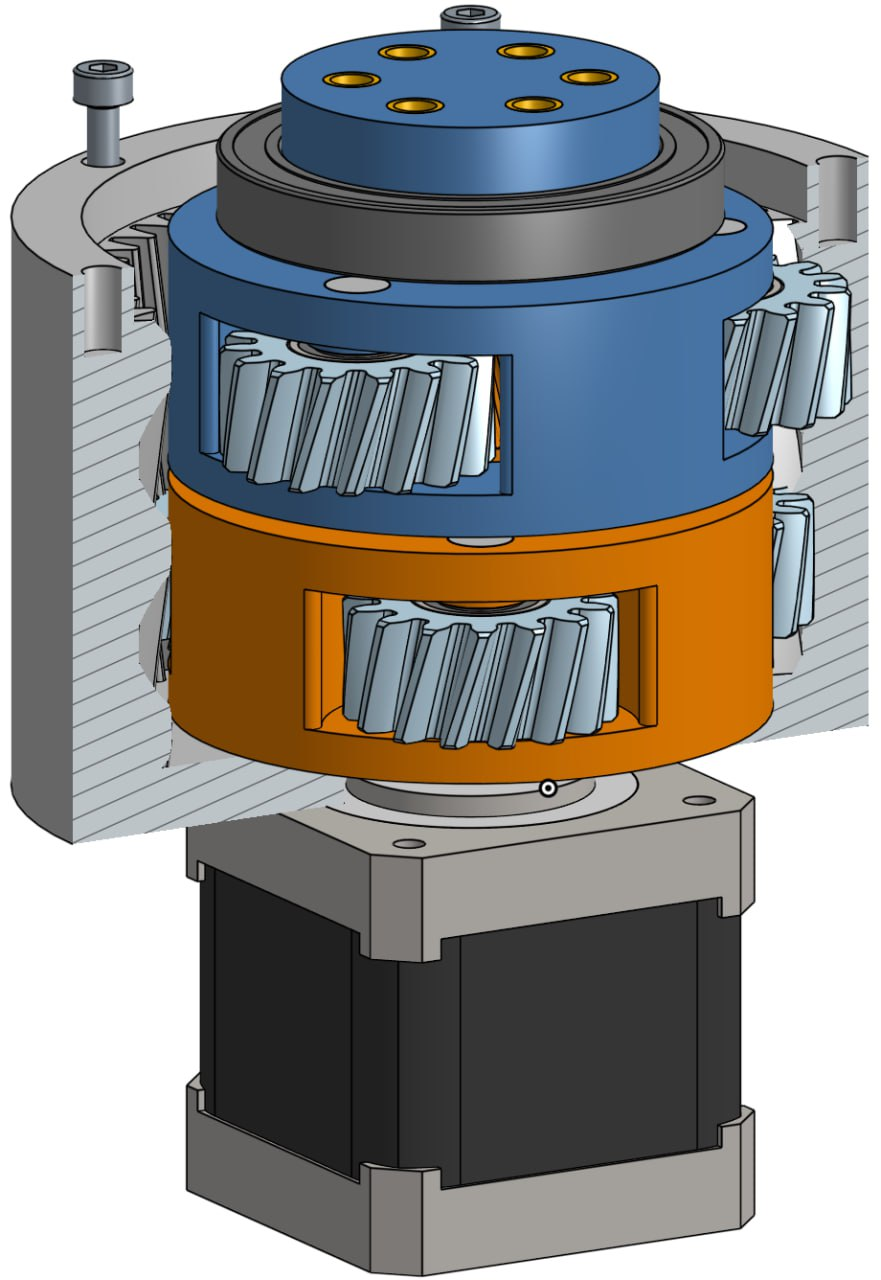
\includegraphics[width=0.4\textwidth]{design/gearbox_design/planetary_gearbox.jpg}
    \caption{Section view of a two-stage planetary gearbox. Illustration taken from \cite{dejan_HowPlanetaryGears_2023}}
    \label{ph:planetary_drive}
\end{figure}
\begin{tabular}{p{0.45\linewidth} p{0.45\linewidth}}
    \textbf{Pros} & \textbf{Cons} \\
    \begin{itemize}[label=\textcolor{green!60!black}{\textbf{+}}]
        \item Symmetric, simple and compact design
        \item Smooth operation can be achieved using helical gears\protect\footnotemark[3].
    \end{itemize}
    &
    \begin{itemize}[label=\textcolor{red!70!black}{\textbf{--}}]
        \item The backlash and noise of the gearbox are strongly influenced by the printing accuracy\footnotemark[4].
    \end{itemize}
\end{tabular}
\footnotetext[3]{The potential drawback in some designs could be the axial forces which arise due to helical nature of teeth. However, for our project this is not an issue since the design of gearbox is vertical.}
\footnotetext[4]{In this project, gears with larger teeth were used in order to reduce the influence of printing tolerances. Although the result shows almost no backlash, it remains quite noisy.}
All things considered, a planetary gearbox is the best solution for our application, featuring both symmetric arrangement of components and simplicity while still providing favourable mechanical characteristics.

\subsection{Choosing Teeth Count}
Unlike with a cycloidal gearbox, it is harder to achieve 9:1 reduction ratio only with one stage while still keeping the overall design compact. Thus, a two-stage design is needed.

Mathematically, planetary gearbox has to satisfy the following equations \cite{_GearSystemsKHK_}:
\begin{equation}
    Z_{\text{ring}} = Z_{\text{sun}} + 2*Z_{\text{planet}},
    \label{eq:geometric_constraint}
\end{equation}
where $Z_{\text{ring}}, Z_{\text{sun}}$ and $Z_{\text{planet}}$ denote the number of teeth of the respective gears. The number of teeth is linearly proportional to the pitch diameter of a gear since they are located at the circumference. Thus, this equation represents a purely geometry constraint required for the sun and ring gears to be able to fit inside the ring gear.
\begin{figure}[H]
    \caption{Visualisation of the geometric constraint defined by \cref{eq:geometric_constraint}\protect\footnotemark[5]. Gears are represented as circles for clarity.}
    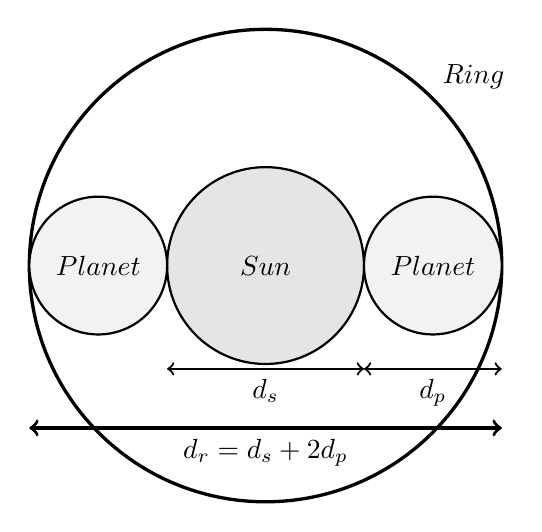
\begin{tikzpicture}[scale=1.25]

\def\rs{1.0}
\def\rp{0.7}
\def\rr{2.4}

\draw[very thick] (0,0) circle (\rr);
\node[above right] at (1.7,1.7) {$\text{Ring}$};

\draw[thick, fill=gray!20] (0,0) circle (\rs);
\node at (0,0) {$\text{Sun}$};

\draw[thick, fill=gray!10] ({\rs+\rp},0) circle (\rp);
\node at ({\rs+\rp},0) {$\text{Planet}$};

\draw[thick, fill=gray!10] ({-(\rs+\rp)},0) circle (\rp);
\node at ({-(\rs+\rp)},0) {$\text{Planet}$};

\draw[<->, thick] (-\rs,-1.05) -- (\rs,-1.05)
    node[midway, below] {$d_{\text{s}}$};

\draw[<->, thick] (\rs,-1.05) -- ({\rs+2*\rp},-1.05)
    node[midway, below] {$d_{\text{p}}$};

\draw[<->, very thick] ({-\rs-2*\rp},-1.65) -- ({\rs+2*\rp},-1.65)
    node[midway, below] {$d_{\text{r}} = d_{\text{s}} + 2d_{\text{p}}$};

\end{tikzpicture}
    \label{fig:gearbox_constraint_tikz}
\end{figure}
\footnotetext[5]{Two planet gears were used for illustration purposes. Our design uses three planet gears, but the constraint condition remains the same.}

The next equation that all planet gears can be placed with equal angular spacing around the sun gear. Equal spacing ensures equal load distribution and helps balance the forces with which planet gears act upon the sun gear.
\begin{equation}
    \frac{Z_{\text{ring}}+Z_{\text{sun}}}{N_{\text{planets}}} = k, k \in \mathbb{N}.
    \label{eq:equal_spacing_constraint}
\end{equation}
If this condition is not fulfilled, the planet gears cannot be equally spaced because proper tooth alignment between the planet gears and the sun/ring gears would not be maintained.

As was already mentioned in \cref{subsubsec:planetary_gearbox}, planetary gearboxes could output different gear ratios depending on which component is fixed and which component is used as the input.
In our case, a ring gear whill be part of the outer shell of the platform, thus it will be stationary. In our case, the following transmission ratio will be true \cite[sec. Fixed ring gear]{tec-science_TransmissionRatiosPlanetary_2021}:
\begin{equation}
    R = 1+\frac{Z_{\text{ring}}}{Z_{\text{sun}}}.
    \label{eq:transmission ratio}
\end{equation}
Considering the constraints given in the \cref{eq:geometric_constraint,eq:equal_spacing_constraint}, for a transmission ratio of 3:1 for one stage, the following teeth counts were chosen:
\begin{equation}
    Z_{\text{ring}} = 64, Z_{\text{sun}} = 32, Z_{\text{planet}} = 16.
\end{equation}